\section{Stage VIII: Moving Polls to Loop Exits --- Counted Loops}
\label{sec:counted}

Two limitations remained: the analysis missed nx's SIMD loops, and the poll
on every back edge rules out interior and carried pointers
(Section~\ref{sec:reality}). A generalised analysis addresses the first,
counted loops the second.

\subsection{Generalising the Address Analysis}
Two patterns hid nx's SIMD loops from the analysis. First, SIMD operations
such as \code{caml_sse2_float64x2_add} reach Cmm as external calls, which
\code{is_gc_free} treated as safepoints; they are \code{[@@noalloc]} builtins
expanded inline, so the check now ignores them. Second, a 128-bit load from
an unboxed float array untags the index with a right shift before scaling,
\code{(+a a (<< (>>s idx 1) 3))}. Writing each index as $y + 2q$, with $q$
a constant, all accesses to one array at the same $y$ should share one
pointer. The identity $(y + 2q) \gg_s 1 = (y \gg_s 1) + q$ holds for
integers but not for 64-bit words: when $y + 2q$ wraps, the two sides differ
by $2^{63}$. The whole byte address is exact nonetheless. With $a$, $y$ and
$q$ 64-bit words read as signed integers and an element of $2^s$ bytes,
$1 \le s \le 3$, the machine computes $w = y + 2q - 2^{64}t$ for some integer
$t$, and $w \gg_s 1 = \lfloor w/2 \rfloor = \lfloor y/2 \rfloor + q -
2^{63}t$ because $2q$ and $2^{64}t$ are even. Scaling by $2^s$ makes the error
$2^{63+s}t$ a multiple of $2^{64}$, so
\[
  a + \bigl(((y + 2q) \gg_s 1) \ll s\bigr) \equiv
  a + \bigl((y \gg_s 1) \ll s\bigr) + (q \ll s) \pmod{2^{64}}
\]
for every $y$ and $q$. The same argument with $2q$ replaced by the counter's
even step $m\cdot n$ shows that a carried pointer advanced by
$(m n / 2) \ll s$ per iteration equals the original address on every
iteration, whatever wraps. The pass also accepts $s = 0$, where the error does
not vanish; there it relies on the original access being in bounds, which an
index whose sum wraps cannot be. With both rules, nx's 8-wide SIMD addition loop shrinks from 52 to 22 instructions
(Listing~\ref{lst:nx-simd}).

\begin{lstlisting}[language=asmX,caption={nx-oxcaml \texttt{add\_float64}, 8-wide SIMD loop, before (24 lea/sar pairs, back-edge poll) and after (one carried pointer per array).},label=lst:nx-simd]
# before (52 instructions, excerpt)
leaq    4(%r10),%rbp
sarq    $1,%rbp                    # untag the index ...
vmovupd (%rsi,%rbp,8),%xmm0        # ... then scale it, for every access
...
addq    $16,%rcx ; addq $16,%rdi ; addq $16,%rax ; addq $16,%rbx
cmpq    (%r14),%r15                # poll on the back edge
jbe     .L393
# after (22 instructions with counted loops)
vmovupd 8(%rax),%xmm0              # constant offsets from carried pointers
vmovupd 8(%r11),%xmm1
vaddpd  %xmm1,%xmm0,%xmm0
vmovupd %xmm0,8(%r10)
...
addq    $64,%r11 ; addq $64,%rax ; addq $64,%r10
\end{lstlisting}

\subsection{Counted Loops}
A loop that is guaranteed to finish and cannot reach the collector can poll
once \emph{after} the loop instead of on every back edge, as a
\code{[@@noalloc]} C call does. No domain is left in an unsafe state, but a
counted loop's time to the next safepoint is its running time. Termination is
essential: a poll-free spin-wait (Listing~\ref{lst:spin}) would stall every
other domain for ever. Under
\code{-cmm-counted-loops}, a GC-free loop with no polled loop inside loses its
back-edge poll if termination is proved, and polls on every exit instead
(Figure~\ref{fig:counted}). Interior and carried pointers are then legal
inside it, since exit values are computed \emph{before} the exit poll. A loop
whose only GC point is on the way out, such as boxing a result, also
qualifies.

A separate two-domain test (three repetitions per case) measures this cost.
One domain repeatedly runs a counted dot product over $N$ floats while a
second allocates and records its longest pause, each minor collection waiting
for the first domain's next safepoint. If the wait is one run of the loop,
the pause should grow with $N$, and it does: with back-edge
polls it stays within the host's jitter (1--4\,ms); with counted loops it
tracks the loop's running time, about 10\,ms for $N = 10^7$ (one run takes
8\,ms) and 74--85\,ms for $N = 10^8$ (70--73\,ms).

\paragraph{A trip cap.} \code{-cmm-counted-loops-max-trips N} (off by
default) keeps the polled copy for any loop that may run more than $N$
iterations. In a later run of the same test with the final passes and a cap
of $10^6$, the worst pause fell from 57--61\,ms to 0.5--1.1\,ms at $N = 10^8$
and from 546--592\,ms to 0.6--2.1\,ms at $N = 10^9$, against 0.4--1.2\,ms
without the pull request. With that cap microgpt runs at $0.848\times$ the
uncapped speed: the cap check reads the loop's start value, so it cannot be
lifted out of an inner loop, and the outer loops of nests lose counted status.

\begin{figure}[h]
  \centering
  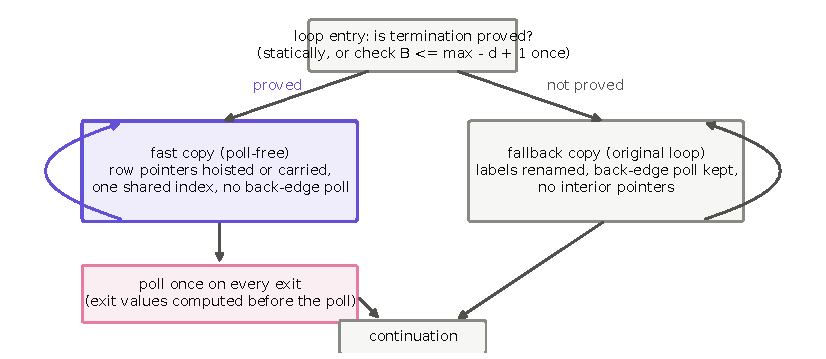
\includegraphics[width=0.86\textwidth]{diag_counted}
  \caption{A counted loop. If termination is not decided at compile time, the
  loop is compiled twice and a single check on entry selects the poll-free
  copy or the original, polled copy.}
  \label{fig:counted}
\end{figure}

\subsection{An Exact Termination Proof}
Loops can wrap around (\code{while i < n do i := i + 16} never ends if
\code{n} is within 15 of \code{max_int}), so the rule is exact in 64-bit
wrapping arithmetic. A loop qualifies when a counter $c$ is stepped by the
same non-zero constant $n$ on every back edge and a test $x \mathrel{R} B$,
with $x = m\cdot c + k$, $m \ne 0$ and $B$ invariant, dominates every back
edge; $x$ then changes by exactly $d = m\cdot n$ per iteration, and the loop
ends under the preconditions of Table~\ref{tab:termination}. Cmm already
holds OCaml integers as tagged machine words, so $c$, $m$, $n$, $k$ and $B$
are machine-word quantities and tagging needs no separate case. The analysis
accepts only $|m|, |d| \le 2^{20}$, which makes $d$ exact and non-zero for
any step below $2^{43}$; a loop whose test does not move ($d = 0$) is never
counted.

\begin{table}[h]
  \centering
  \small
  \begin{tabular}{@{}ll@{}}
    \toprule
    loop continues while & proved to terminate when \\
    \midrule
    $x < B$, $d > 0$ & $B \le \textit{max} - d + 1$ \\
    $x \le B$, $d > 0$ & $B \le \textit{max} - d$ \\
    $x > B$, $d < 0$ & $B \ge \textit{min} - d - 1$ \\
    $x \ge B$, $d < 0$ & $B \ge \textit{min} - d$ \\
    $x \ne B$, $|d| = 2^k$ & $x_0 \le B$ and $(B - x_0) \bmod |d| = 0$ (mirrored for $d < 0$) \\
    $x = B$, $d \ne 0$ & always (the test fails by the second iteration) \\
    anything else & never \\
    \bottomrule
  \end{tabular}
  \caption{Termination preconditions. For example, $i \ne n$ stepping by 2
  never ends if $n - i$ is odd.}
  \label{tab:termination}
\end{table}

A small interval analysis decides the precondition at compile time where it
can (microgpt's trip count \code{(cols - 2) >> 1} can never approach
\code{max_int}); otherwise one check on entry selects between two copies of
the loop. Checks that depend only on outer-loop invariants are lifted
outward, making a nest one poll-free region behind one check; nests inside
loops that still poll get no exit polls, since the enclosing poll bounds the
time to the next safepoint. A size budget limits the fallback copies: a
12-deep nest's code shrinks from 5,712 to 2,912 bytes, and microgpt is
unchanged. \code{-dcounted-loops} prints each loop's decision and reason.

\paragraph{Why it is safe.} A derived pointer is never live across a GC
point, because interior and carried pointers form only in loops with no
allocation, call or poll. The backend's \code{bad GC root} check rejects any
violation at compile time. Other domains' stop-the-world sections need this
domain to poll, which it does at loop exit. The collector is not idle
meanwhile: other domains may mark and sweep the major heap concurrently.
Marking never moves an object, and sweeping frees only objects that were
unreachable when the major cycle began, which the loop's arrays were not.
What moves objects, minor collections and compaction, is stop-the-world in
OCaml~5 and so must wait until this domain reaches a safepoint; no object a
derived pointer points into can move while the loop runs. The termination proof is exact in 64-bit wrapping
arithmetic, so every counted loop reaches its exit poll. These are two
guarantees: the collector never sees a derived pointer, and every domain
eventually polls. A third, a bound on how long another domain waits, does not
follow from termination; that is the latency measured above, and the trip cap
bounds iterations without a poll, not their running time.

\subsection{Unchecked Loops}
My guide asked for a variant without the termination proof.
\code{-cmm-unchecked-loops} gives every GC-free loop the optimisation and also
drops back-edge polls in loops that contain calls; on microgpt it makes 78 of
the 86 loops poll-free (the other 8 contain an exception handler). Apparent
spin-waits (loops containing \code{Domain.cpu_relax} or an atomic) keep their
poll; loops with a tail call or an exception handler get no exit poll; and the
runtime's never-polled method-dispatch helpers are skipped in both modes. A
loop waiting on a plain mutable field loses its poll, so the mode stays opt-in
(Section~\ref{sec:liveness}).

\subsection{Giving Up Liveness}
\label{sec:liveness}
Three builds remove polls from loops without a termination proof
(Table~\ref{tab:liveness}). Their output is correct, but their loops can no
longer be preempted, and a loop that waits on another domain or a signal may
never terminate. None beats counted loops by more than about the run's
resolution: once the pointer passes can act, the remaining polls cost little,
and on the release, removing polls without the passes gains little.

\begin{table}[h]
  \centering
  \small
  \begin{tabular}{@{}llrrr@{}}
    \toprule
    build & polls removed by & tokens/s & vs scalar C++ & vs \code{pr_counted} \\
    \midrule
    \code{pr_unchecked} & \code{-cmm-unchecked-loops} & 585,497 & $1.22\times$ & $+3.3\%$ (17/21) \\
    \code{pr_nopoll} & \code{-disable-poll-insertion} & 577,723 & $1.24\times$ & $+1.2\%$ (13/21) \\
    \code{oxcaml_unsafe_unroll_pollfree} & the same, on the release &441,269 & $1.62\times$ & $-19.6\%$ (0/21) \\
    \bottomrule
  \end{tabular}
  \caption{Builds that give up liveness (run W, generation mode; the last
  column is the paired change against the counted build).}
  \label{tab:liveness}
\end{table}

\subsection{Verification}
The rebased pull request was checked against an unpatched build of the same
commit. The upstream test suite (2,973 tests) gives the same result test by
test with default flags; with the new flags forced onto every test through
\code{OCAMLPARAM}, only expected tests change (Table~\ref{tab:testsuite}):
two because \code{[@poll error]} functions may now contain counted loops, and
in unchecked mode 16 preemption tests and 2 newer thread-local-storage tests
that wait for preemption ticks, the expected loss of liveness.

\begin{table}[h]
  \centering
  \small
  \begin{tabular}{@{}lrrl@{}}
    \toprule
    mode (155 tests skipped in each) & passed & failed & failures \\
    \midrule
    unpatched compiler & 2,818 & 0 & \\
    defaults (four passes on) & 2,818 & 0 & identical to unpatched \\
    \code{-cmm-counted-loops} & 2,816 & 2 & the two \code{[@poll error]} tests \\
    \code{-cmm-unchecked-loops} & 2,800 & 18 & 16 preemption, 2 thread-local storage \\
    \bottomrule
  \end{tabular}
  \caption{The upstream OxCaml test suite on the rebased pull-request
  compiler, configured like the release.}
  \label{tab:testsuite}
\end{table}

Adversarial tests target what the suite does not. Fifteen deliberately
non-terminating loop shapes stay interruptible under counted loops: no false
termination proof. Eight test programs, built with eight flag
configurations, with and without \code{-unsafe}, and run under GC stress,
effects and extra domains, print what the unpatched compiler prints in every
combination except the four expected hangs of non-terminating loops in builds
with polls removed. microgpt's hot loop is unchanged by the rebase (13
instructions per 4 multiply--adds, no poll). Earlier versions also passed all
963 nx-oxcaml tests and the 915 single-file programs of OxCaml's test
directories in three modes. The pull request is on my OxCaml
fork~\cite{oxcaml_pr}; the new loop flags are off by default.

\subsection{Results}
On microgpt, counted loops are worth $+16.6\%$ (21/21) over the four
passes with polls on every back edge. Table~\ref{tab:counted} and
Figure~\ref{fig:nxops} give nx-oxcaml.

\begin{table}[h]
  \centering
  \small
  \begin{tabular}{@{}lrrl@{}}
    \toprule
    workload & speed-up & rounds & \\
    \midrule
    nx element-wise (9 cases) & $1.70$--$2.89\times$ & 21/21 each & \\
    nx full reduction, sum f64 32,768 & $1.34\times$ & 21/21 & \\
    nx matrix multiply (7 cases) & $1.01$--$1.11\times$ & 14--20/21 & \\
    \midrule
    hot-loop instructions & without & with & \\
    \midrule
    microgpt \code{linear} (4 rows) & 22 & 13 & \\
    nx \code{add_float64} (8-wide SIMD) & 52 & 22 & \\
    nx GEMM micro-kernel & 41 & 33 & \\
    \bottomrule
  \end{tabular}
  \caption{\texttt{-cmm-counted-loops} against the same compiler without it,
  polls and the four passes on in both (separate nx runs of 21 rounds, median
  of per-round ratios; no case became slower).}
  \label{tab:counted}
\end{table}

\begin{figure}[h]
  \centering
  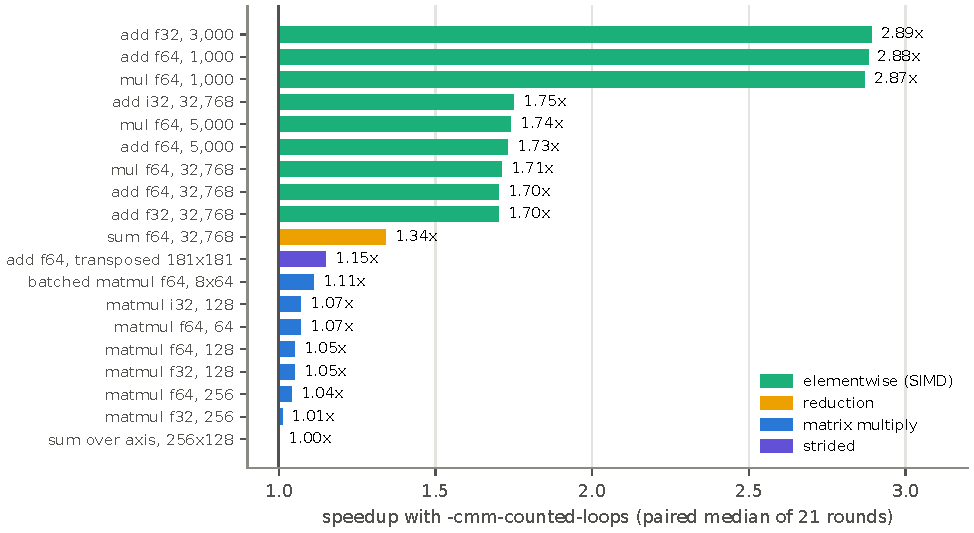
\includegraphics[width=0.86\textwidth]{fig_nx_ops}
  \caption{nx-oxcaml, every benchmarked operation, counted loops versus the same
  compiler without them (21 rounds, polls on in both).}
  \label{fig:nxops}
\end{figure}

The spread follows from what the pass removes. Only 4 of the 22 loop
instructions of an element-wise addition are arithmetic; at 1,000 elements
instruction count sets the speed ($2.9\times$), at 32,768 memory starts to
limit it ($1.7\times$). Matrix multiply is almost pure arithmetic.

This comparison mixes two changes: counted loops remove the back-edge polls,
and the generalised analysis lets the pointer passes act on nx's SIMD loops at
all. A second nx run (21 rounds, identical results in every arm) changes one
thing at a time (Table~\ref{tab:nxablation}). Removing polls with the pointer
passes off measures the polls' own cost: a few percent. The pointer passes in
builds without polls measure the analysis alone: most of the gain. Counted
loops match that poll-free build. The speed-up therefore comes from the
generalised analysis; moving the polls lets it act. With default
flags the final passes run these kernels at the speed of the passes-off build
(Section~\ref{sec:sr-pass}), so counted loops are worth $1.42$--$2.43\times$
over either.

\begin{table}[h]
  \centering
  \small
  \begin{tabular}{@{}lr@{}}
    \toprule
    nx element-wise kernels (9 cases), paired speed-up & range \\
    \midrule
    removing polls, pointer passes off & $1.04$--$1.08\times$ \\
    pointer passes, both builds without polls & $1.60$--$2.58\times$ \\
    counted loops against removing every poll & $0.97$--$1.01\times$ \\
    counted loops against passes off & $1.42$--$2.43\times$ \\
    \midrule
    final passes, defaults against the defaults measured above & $1.10$--$1.14\times$ \\
    final passes, counted loops against counted loops above & $0.99$--$1.01\times$ \\
    \bottomrule
  \end{tabular}
  \caption{What the nx-oxcaml speed-ups are made of (separate 21-round run,
  single domain; two byte-identical builds differed by about 1\%). The last two
  rows are a later 15-round run with the final passes.}
  \label{tab:nxablation}
\end{table}

\subsection{How Close Is Counted to Poll-Free?}
\label{sec:last2}
Removing polls altogether is worth $+1.2\%$ (13/21) over the counted
build (interquartile range $[-0.8, +7.4]\%$), within run W's
resolution (byte-identical copies differ by $+0.6\%$,
$[-0.2, +2.9]\%$).

Of the four polls left in \code{linear} (row-group loop exit, function exit,
fallback copy), each call executes two, never taken, outside every loop.
After normalising addresses, \code{linear}'s 42-instruction row-group loop is
identical to that of a build with no polls. Outside it, the counted build
keeps a stack frame in \code{linear} and carries the fallback loops
(\code{linear} grows from 107 to 215 instructions, \code{forward} from 582 to
777). Overwriting every remaining poll with NOPs (Section~\ref{sec:polls})
changed nothing measurable in a separate test.

The obvious remaining candidate is code layout: if a loop's address alone
moves a build by as much as the builds differ, no difference can be credited
to the polls or to loop versioning. A separate test relinked the counted,
unchecked and poll-free builds at four code addresses each, \code{linear}'s
instructions identical in all twelve (21 rounds). Moving the code changed each
build's speed by 2--3.5\%, while averaged over the four layouts the three
builds differ by at most 0.4\%, and which is fastest depends on the layout.
Counted loops are therefore as fast as removing polls altogether.

\subsection{What Counted Loops Cost}
The final compiler counts 39 of microgpt's 85 loops: 25 proved at compile
time and 14 guarded by an entry check (two copies). The other 46 are rejected:
39 contain a GC point, 6 have no exit test dominating the back edges, and 1
has an inner entry check that could not be lifted. The module's machine code grows
by 2.1\% (58,817 to 60,059 bytes) and the whole binary by 0.07\%. Build time
is unchanged (medians 2.29--2.31\,s over seven interleaved builds).
